% Indradhanu V1 (v0.2.0) against V2 (Heavy, v2.1.0), in the grouped/hatched style; V2's new parts outlined in ochre.
% Sources: docs/04-models.md (V1: 165-band grid, 1x1 compressor to 24-32 channels, SegFormer MAE, pixel-shuffle decoder, 5.5 M;
% V2: wavelength stem, [96,192,480,768], heads [3,6,10,12], progressive decoder 512 -> 256/128, 35.3 M);
% docs/lld/spectral-stem.md (40 nm bins, per-band skip, thick-cloud rule); research/textbook/chapters/41-heavy.tex (33,884,194 + 1,431,120).
\adjustbox{max width=\textwidth, max totalheight=0.53\textheight}{%
\begin{tikzpicture}[x=1mm,y=1mm]
% ---------------- V1 ----------------
\node[grp, fill=pB!35, minimum width=176mm, minimum height=24mm, anchor=north west] (G1) at (0,0) {};
\node[glab] at (G1.north west) {Indradhanu V1 (v0.2.0) \textperiodcentered{} 5.5\,M parameters \textperiodcentered{} a spatial model: 165 resampled bands are fixed input channels};
\node[inner sep=0, anchor=west] (i1) at (4,-13) {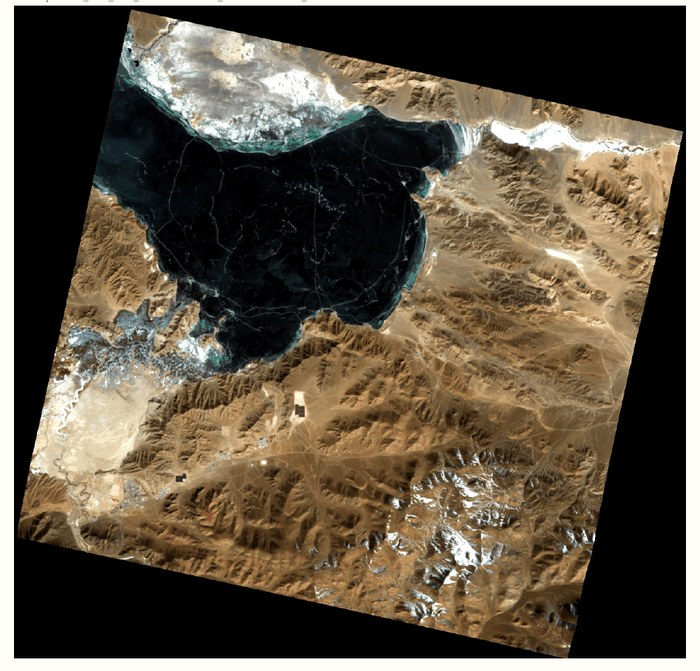
\includegraphics[width=12mm]{figures/story_prisma_k1.jpg}};
\node[tsh, below=0.3mm of i1] {165-band grid};
\node[stg, minimum width=15mm, minimum height=10mm] (c1) at (31,-13) {1$\times$1\\compressor};
\node[tsh, above=0.4mm of c1] {165 $\to$ 24--32 ch};
\node[grp, fill=pG!30, minimum width=58mm, minimum height=17mm] (E1) at (75,-13.5) {};
\node[glab] at (E1.north west) {Encoder};
\foreach \i/\x in {1/53,2/67,3/81,4/95} {
  \node[stg, minimum width=11mm, minimum height=9mm] (s1\i) at (\x,-14.5) {};
  \node[font=\itshape\fontsize{6}{7}\selectfont] at (\x,-12.2) {stage \i};
  \node[cell, fill=pG] at (\x-1.4,-16.4) {}; \node[cell, fill=pG] at (\x+1.4,-16.4) {};}
\foreach \i [evaluate=\i as \j using int(\i+1)] in {1,2,3} \draw[df] (s1\i) -- (s1\j);
\node[grp, fill=pY!35, minimum width=20mm, minimum height=17mm] (D1) at (120,-13.5) {};
\node[glab] at (D1.north west) {Decoder};
\node[stg, minimum width=14mm, minimum height=9mm] (d1) at (120,-14.5) {SegFormer\\pixel shuffle};
\node[font=\fontsize{7}{8}\selectfont] (o1) at (143,-13) {$\hat{\mathbf x}$};
\node[loss] (l1) at (156,-8) {L1 + SAM};
\node[loss] (r1) at (156,-18) {combined score};
\draw[df] (i1) -- (c1); \draw[df] (c1) -- (s11); \draw[df] (s14) -- (d1); \draw[df] (d1) -- (o1);
\draw[tf] (o1) -- (l1); \draw[df] (o1) -- (r1);
% ---------------- V2 ----------------
\node[grp, fill=pR!30, minimum width=176mm, minimum height=40mm, anchor=north west] (G2) at (0,-28) {};
\node[glab] at (G2.north west) {Indradhanu V2 (v2.1.0, Heavy) \textperiodcentered{} 33.9\,M + 1.43\,M head = 35.3\,M parameters \textperiodcentered{} spectral: bands enter as (value, wavelength)};
\node[inner sep=0, anchor=west] (i2) at (4,-46) {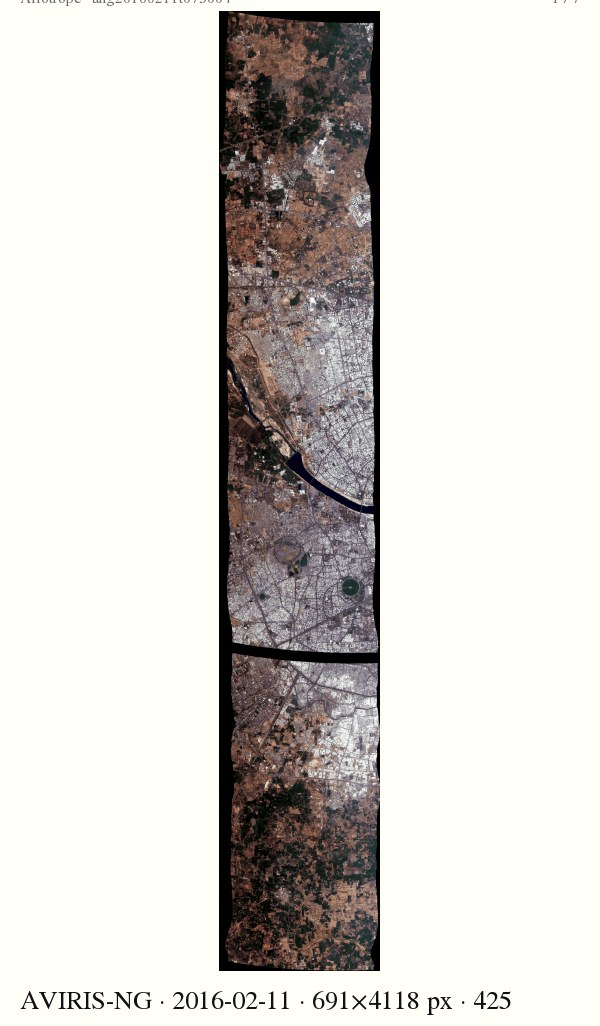
\includegraphics[width=12mm]{figures/story_aviris_k1.jpg}};
\draw[ochre!85!black, line width=0.6pt] plot[smooth] coordinates {(4,-60) (6,-58.2) (8,-57.5) (9.5,-59.5) (11,-56.8) (13,-57.3) (16,-58.6)};
\node[tsh, text=ochre!80!black] at (10,-62.5) {any bands, native};
% stem
\node[grp, fill=pY!30, draw=ochre!85!black, solid, minimum width=30mm, minimum height=26mm] (S2) at (37,-47) {};
\node[glab] at (S2.north west) {Spectral stem};
\foreach \k in {0,...,6} \node[cell, fill=pY] at (26.5+\k*2.9,-42.4) {};
\node[tsh] at (35.2,-39.8) {40\,nm wavelength bins};
\foreach \k in {0,...,3} \node[cell, circle, fill=pB] at (30.8+\k*2.9,-47.5) {};
\node[tsh] at (35.2,-51) {attention, 4 heads};
\node[stgn, minimum width=13mm, minimum height=4.5mm] (z2) at (35.2,-56.4) {64 ch};
\draw[df] (35.2,-43.6) -- (35.2,-45.8); \draw[df] (35.2,-49.2) -- (z2);
% encoder
\node[grp, fill=pG!30, draw=ochre!85!black, solid, minimum width=62mm, minimum height=26mm] (E2) at (90,-47) {};
\node[glab] at (E2.north west) {Encoder, 3$\times$ wider};
\foreach \i/\x/\w/\c/\h in {1/68/8/96/3,2/80/10/192/6,3/94/12.5/480/10,4/110/15/768/12} {
  \node[stgn, minimum width=\w mm, minimum height=11mm] (s2\i) at (\x,-48) {};
  \node[font=\itshape\fontsize{6}{7}\selectfont] at (\x,-45.2) {stage \i};
  \node[cell, fill=pG] at (\x-1.4,-49) {}; \node[cell, fill=pG] at (\x+1.4,-49) {};
  \node[font=\itshape\fontsize{5.2}{6}\selectfont] at (\x,-51.6) {\c, \h\ h};}
\foreach \i [evaluate=\i as \j using int(\i+1)] in {1,2,3} \draw[df] (s2\i) -- (s2\j);
% decoder
\node[grp, fill=pY!30, draw=ochre!85!black, solid, minimum width=24mm, minimum height=26mm] (D2) at (138,-47) {};
\node[glab] at (D2.north west) {Decoder};
\node[stgn, minimum width=18mm, minimum height=5mm] (u1) at (138,-43.5) {fuse 512 $\to$ 256};
\node[stgn, minimum width=18mm, minimum height=5mm] (u2) at (138,-52.5) {up 256 $\to$ 128};
\draw[df] (u1) -- (u2);
% heads
\node[font=\fontsize{7}{8}\selectfont] (o2) at (158,-40) {$\hat{\mathbf x}$};
\node[loss] (l2) at (173,-36) {L1 + SAM};
\node[loss] (r2) at (173,-44.5) {Mahalanobis};
\node[stgn, minimum width=13mm, minimum height=7mm] (h2) at (164,-58) {seg head};
\node[tsh] at (164,-63.6) {land water cloud shadow snow};
\node[loss] (b2) at (176,-52) {BCE+Dice};
% flows
\draw[df] (i2) -- (S2.west |- i2); \draw[df] (z2.east) -- (s21.west |- z2.east) ;
\draw[df] (s24) -- (u1.west |- s24);
\draw[df] (u2.east) -| (o2.south);
\draw[tf] (o2) -- (l2); \draw[df] (o2) -- (r2);
\draw[tf, draw=ochre!85!black] (s24.north) -- (110,-31.5) -| (h2.north);
\draw[tf] (h2) -- (b2);
\draw[tf] (z2.south) -- ++(0,-6.5) -| node[pos=0.3, tsh, above]{skip at full resolution, hidden pixels zeroed} (u2.south);
% ---------------- legend ----------------
\begin{scope}[shift={(4,-75)}]
\node[stg, minimum width=7mm, minimum height=3.5mm] at (3,0) {}; \node[tsh, anchor=west, text=ink] at (7.5,0) {stage block};
\node[cell, fill=pG] at (30,0) {}; \node[cell, fill=pY] at (32.5,0) {}; \node[cell, circle, fill=pB] at (35,0) {}; \node[tsh, anchor=west, text=ink] at (37,0) {cells: transformer blocks, wavelength bins, attention heads};
\node[loss] at (101,0) {loss}; \node[tsh, anchor=west, text=ink] at (105,0) {loss / score};
\draw[df] (124,0) -- (131,0); \node[tsh, anchor=west, text=ink] at (132,0) {data flow};
\draw[tf] (147,0) -- (154,0); \node[tsh, anchor=west, text=ink] at (155,0) {training-only / optional};
\draw[ochre!85!black, line width=0.9pt, rounded corners=1pt] (-1,-4.5) rectangle (6,-2.6); \node[tsh, anchor=west, text=ink] at (7.5,-3.6) {new in V2};
\end{scope}
\end{tikzpicture}}
